\documentclass[]{article}
\usepackage{lmodern}
\usepackage{amssymb,amsmath}
\usepackage{ifxetex,ifluatex}
\usepackage{fixltx2e} % provides \textsubscript
\ifnum 0\ifxetex 1\fi\ifluatex 1\fi=0 % if pdftex
  \usepackage[T1]{fontenc}
  \usepackage[utf8]{inputenc}
\else % if luatex or xelatex
  \ifxetex
    \usepackage{mathspec}
  \else
    \usepackage{fontspec}
  \fi
  \defaultfontfeatures{Ligatures=TeX,Scale=MatchLowercase}
\fi
% use upquote if available, for straight quotes in verbatim environments
\IfFileExists{upquote.sty}{\usepackage{upquote}}{}
% use microtype if available
\IfFileExists{microtype.sty}{%
\usepackage{microtype}
\UseMicrotypeSet[protrusion]{basicmath} % disable protrusion for tt fonts
}{}
\usepackage[margin=1in]{geometry}
\usepackage{hyperref}
\hypersetup{unicode=true,
            pdftitle={Análisis de conglomerados},
            pdfauthor={Dra. Rocío Maehara},
            pdfborder={0 0 0},
            breaklinks=true}
\urlstyle{same}  % don't use monospace font for urls
\usepackage{graphicx,grffile}
\makeatletter
\def\maxwidth{\ifdim\Gin@nat@width>\linewidth\linewidth\else\Gin@nat@width\fi}
\def\maxheight{\ifdim\Gin@nat@height>\textheight\textheight\else\Gin@nat@height\fi}
\makeatother
% Scale images if necessary, so that they will not overflow the page
% margins by default, and it is still possible to overwrite the defaults
% using explicit options in \includegraphics[width, height, ...]{}
\setkeys{Gin}{width=\maxwidth,height=\maxheight,keepaspectratio}
\IfFileExists{parskip.sty}{%
\usepackage{parskip}
}{% else
\setlength{\parindent}{0pt}
\setlength{\parskip}{6pt plus 2pt minus 1pt}
}
\setlength{\emergencystretch}{3em}  % prevent overfull lines
\providecommand{\tightlist}{%
  \setlength{\itemsep}{0pt}\setlength{\parskip}{0pt}}
\setcounter{secnumdepth}{0}
% Redefines (sub)paragraphs to behave more like sections
\ifx\paragraph\undefined\else
\let\oldparagraph\paragraph
\renewcommand{\paragraph}[1]{\oldparagraph{#1}\mbox{}}
\fi
\ifx\subparagraph\undefined\else
\let\oldsubparagraph\subparagraph
\renewcommand{\subparagraph}[1]{\oldsubparagraph{#1}\mbox{}}
\fi

%%% Use protect on footnotes to avoid problems with footnotes in titles
\let\rmarkdownfootnote\footnote%
\def\footnote{\protect\rmarkdownfootnote}

%%% Change title format to be more compact
\usepackage{titling}

% Create subtitle command for use in maketitle
\providecommand{\subtitle}[1]{
  \posttitle{
    \begin{center}\large#1\end{center}
    }
}

\setlength{\droptitle}{-2em}

  \title{\textbf{Análisis de conglomerados}}
    \pretitle{\vspace{\droptitle}\centering\huge}
  \posttitle{\par}
    \author{Dra. Rocío Maehara}
    \preauthor{\centering\large\emph}
  \postauthor{\par}
      \predate{\centering\large\emph}
  \postdate{\par}
    \date{23 de noviembre de 2019}


\begin{document}
\maketitle

\subsection{Introducción}\label{introducciuxf3n}

Supóngase que el responsable de marketing de una empresa tiene una base
de datos con las {características sociodemográficas de sus clientes}:
{edad}, {nivel educativo}, {nivel de ingresos}, {estado civil}, {tipo de
ocupación}, {número de hijos}, etc. Este directivo se plantea si podría
{dividir a sus clientes en subgrupos}, que tuvieran {características
sociodemográficas similares entre sí}, pero que {unos subgrupos de
otros}, fueran {lo más diferentes posibles}.

\subsection{Introducción}\label{introducciuxf3n-1}

Si esto fuera posible, el directivo de marketing podría, por ejemplo,
{diseñar campañas de publicidad distintas para cada grupo}, con
{creatividades diferentes} o {utilizando diarios, revistas o cadenas de
televisión distintas} según el grupo al que fuera dirigida la campaña.

\subsection{Introducción}\label{introducciuxf3n-2}

E{]} análisis de conglomerados, al que también se denomina comúnmente
análisis cluster, es una técnica diseñada para clasificar distintas
observaciones en grupos, de tal forma que:

\begin{itemize}
\item
  Cada grupo (conglomerado o cluster) sea homogéneo respecto a las
  variables utilizadas para caracterizarlo, es decir, que cada
  observación contenida en él sea parecida a todas las que estén
  incluidas en ese grupo.
\item
  Que los grupos sean lo más distintos posible unos de otros respecto a
  las variables consideradas.
\end{itemize}

\subsection{Introducción}\label{introducciuxf3n-3}

Es importante señalar, para distinguir el análisis de conglomerados de
otras técnicas tratadas anteriormente, que los grupos son desconocidos a
priori y es necesario derivarlos de las observaciones. En el análisis
discriminante o la regresión logística, por ejemplo, las observaciones
ya estan previamente clasificadas en dos o más grupos, buscándose las
razones que explican esa clasificación y no la clasificación en sí.

\subsection{Proceso del análisis de
conglomerados}\label{proceso-del-anuxe1lisis-de-conglomerados}

\hypertarget{left}{}
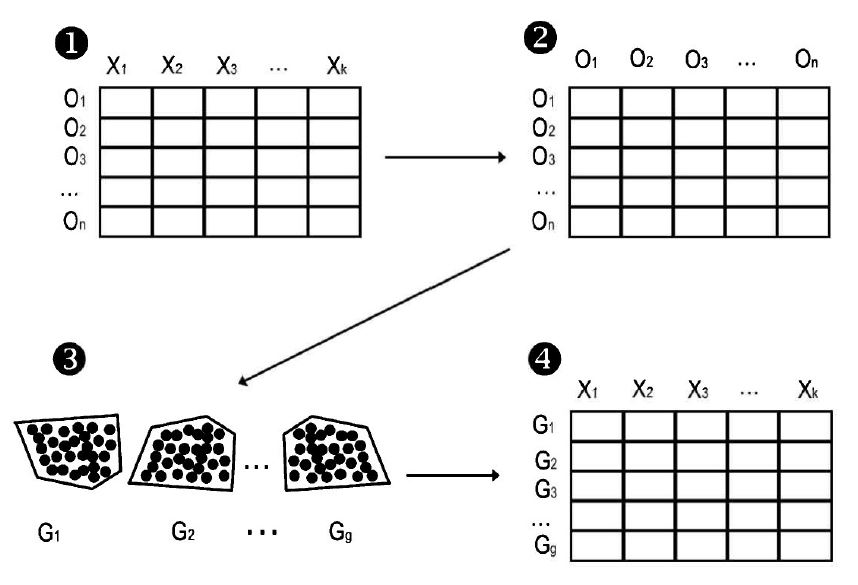
\includegraphics[width=1\linewidth]{images/proc_congl}

\hypertarget{right}{}
\begin{itemize}
\item
  Inicialmente, el investigador dispone de \(n\) observaciones
  (individuos, empresas, etc.) de las que tiene información sobre \(k\)
  variables (edad, estado civil, número de hijos\ldots{}).
\item
  A continuación, se establece un indicador que nos diga en qué medida
  cada par de observaciones se parece entre sí. A esta medida se la
  denomina distancia o (di)similaridad.
\end{itemize}

\subsection{Proceso del análisis de
conglomerados}\label{proceso-del-anuxe1lisis-de-conglomerados-1}

\hypertarget{left}{}
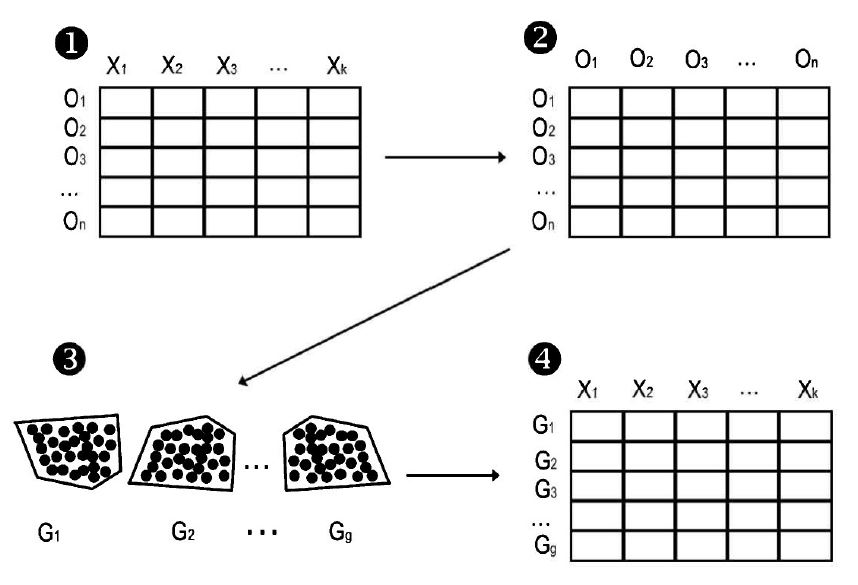
\includegraphics[width=1\linewidth]{images/proc_congl}

\hypertarget{right}{}
\begin{itemize}
\tightlist
\item
  Consiste en hacer grupos con aquellas observaciones que mas se
  parezcan entre sí, de acuerdo con la medida de similaridad calculada
  anteriormente. Ello exige elegir entre los dos tipos de análisis de
  conglomerados: jerárquico y no jerárquico y el método de
  conglomeración para el tipo de análisis elegido (centroide o vecino
  mas cercano, entre otros, en el conglomerado jerárquico).
\end{itemize}

\subsection{Proceso del análisis de
conglomerados}\label{proceso-del-anuxe1lisis-de-conglomerados-2}

\hypertarget{left}{}
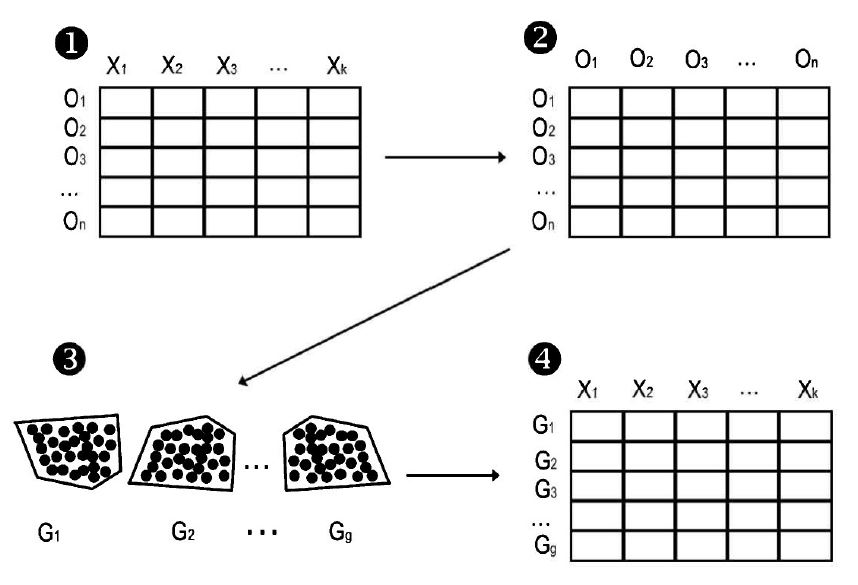
\includegraphics[width=1\linewidth]{images/proc_congl}

\hypertarget{right}{}
\begin{itemize}
\tightlist
\item
  Finalmente, el investigador debe describir los grupos que ha obtenido
  y comparar los unos con los otros. Para ello bastará con ver qué
  valores promedio toman las \(k\) variables utilizadas en el análisis
  de conglomerados en cada uno de los \(g\) grupos obtenidos
  (\(g < n\)).
\end{itemize}

\subsection{Ejemplo}\label{ejemplo}

\textbf{Relación entre la publicidad y las ventas } Supongamos que un
investigador tiene información del presupuesto que un conjunto de
empresas ha destinado a publicidad el ultimo año y de las ventas que han
logrado. Puede preguntarse si estas empresas pueden agruparse en función
de la rentabilidad en términos de ventas que han sido capaces de generar
con su inversión publicitaria.

\subsection{Ejemplo}\label{ejemplo-1}

\textbf{Relación entre la publicidad y las ventas } Por ejemplo, el
investigador puede examinar si existe un grupo de empresas que,
invirtiendo en publicidad relativamente poco, ha logrado una elevada
cifra de ventas o, por el contrario, si existe un grupo que, aun
invirtiendo mucho en publicidad, no ha sido capaz de vender tanto como
sus competidoras. En definitiva, ¿qué tipologia de empresas puede
establecerse en función de la rentabilidad obtenida de su inversión
publicitaria?

\subsection{Ejemplo}\label{ejemplo-2}

\begin{verbatim}
Empresa <- c("E1","E2","E3","E4","E5","E6","E7","E8")
Inversion_publicitaria <- c(16,12,10,12,45,50,45,50)
Ventas <- c(10,14,22,25,10,15,25,27)
datos <- data.frame(Inversion_publicitaria,Ventas)
attach(datos)
row.names(datos)<-Empresa
plot(Inversion_publicitaria,Ventas,pch=16,xlab="Inversión",ylab="Ventas",xlim=c(5,60),ylim=c(5,30))
with(datos, text(Ventas~Inversion_publicitaria, labels = row.names(datos), pos = 4))


\end{verbatim}

\subsection{Ejemplo}\label{ejemplo-3}

\hypertarget{left}{}
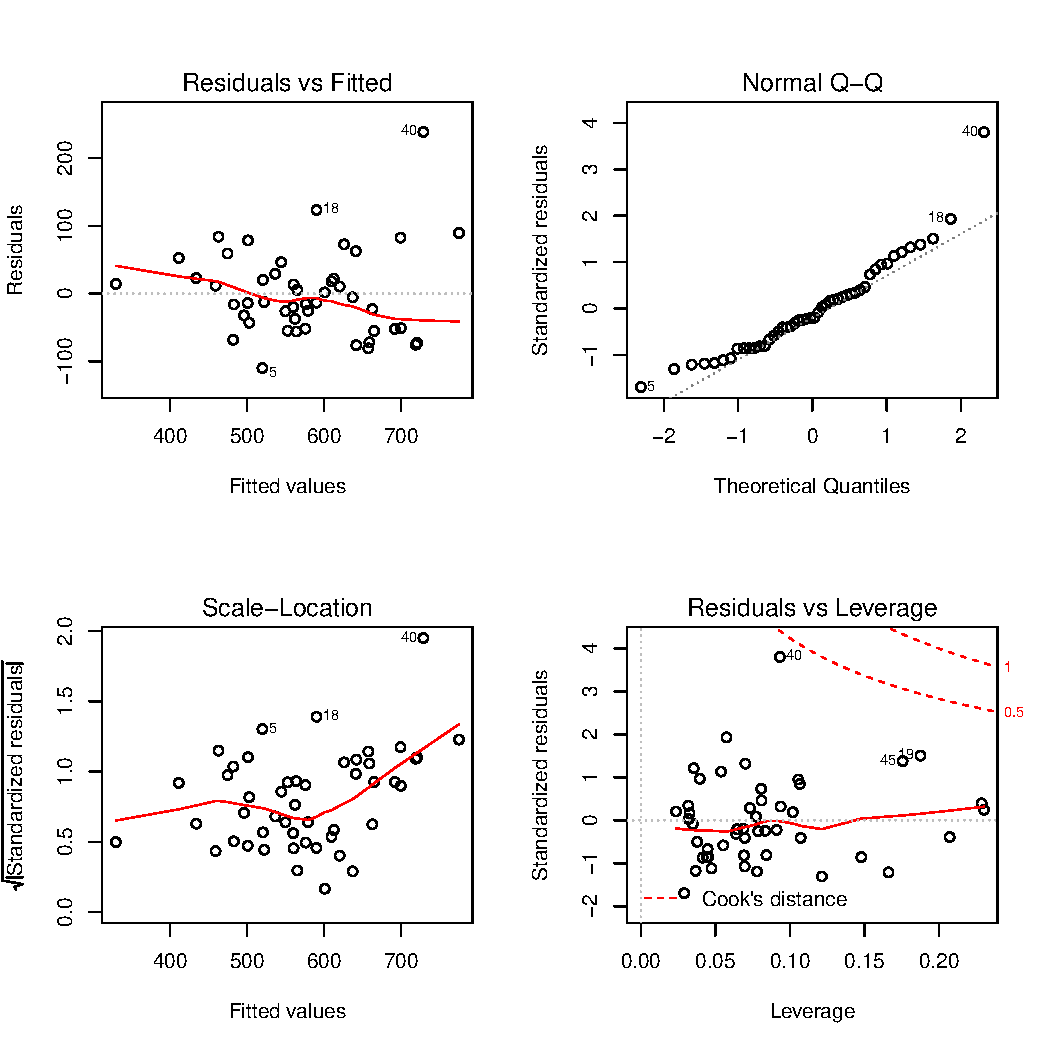
\includegraphics{Clase-6_files/figure-latex/unnamed-chunk-4-1.pdf}

\hypertarget{right}{}
Al haber utilizado solo dos variables en el ejemplo planteado, este
gráfico permite responder de una manera intuitiva a las preguntas que se
hace el investigador. A la vista de este gráfico pueden distinguirse
cuatro grupos de empresas:

\begin{itemize}
\tightlist
\item
  El grupo formado porlas empresas E1 y E2, que, con una pequeña
  inversión en publicidad, han obtenido también pocas ventas.
\end{itemize}

\subsection{Ejemplo}\label{ejemplo-4}

\hypertarget{left}{}
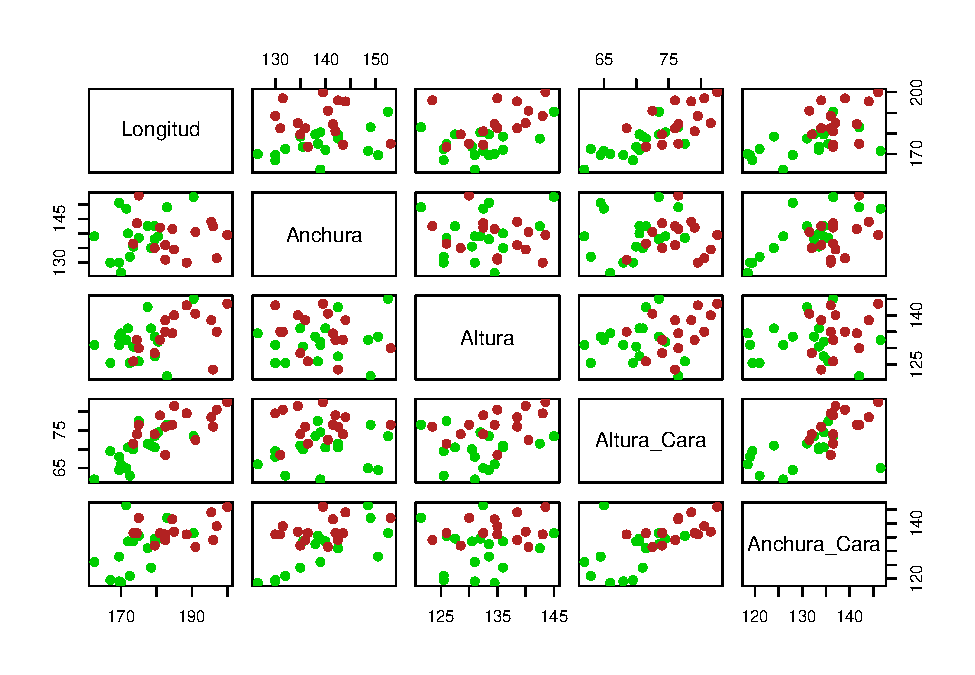
\includegraphics{Clase-6_files/figure-latex/unnamed-chunk-5-1.pdf}

\hypertarget{right}{}
\begin{itemize}
\item
  El grupo formado por las empresas E3 y E4, que, pese a haber invertido
  tan poco como las empresas del grupo anterior, han obtenido una gran
  rentabilidad en términos de ventas a estas inversiones.
\item
  El grupo formado por las empresas E5 y E6, que, pese a haber efectuado
  un gran esfuerzo publicitario, no han sido capaces de obtener unas
  ventas razonables.
\end{itemize}

\subsection{Ejemplo}\label{ejemplo-5}

\hypertarget{left}{}
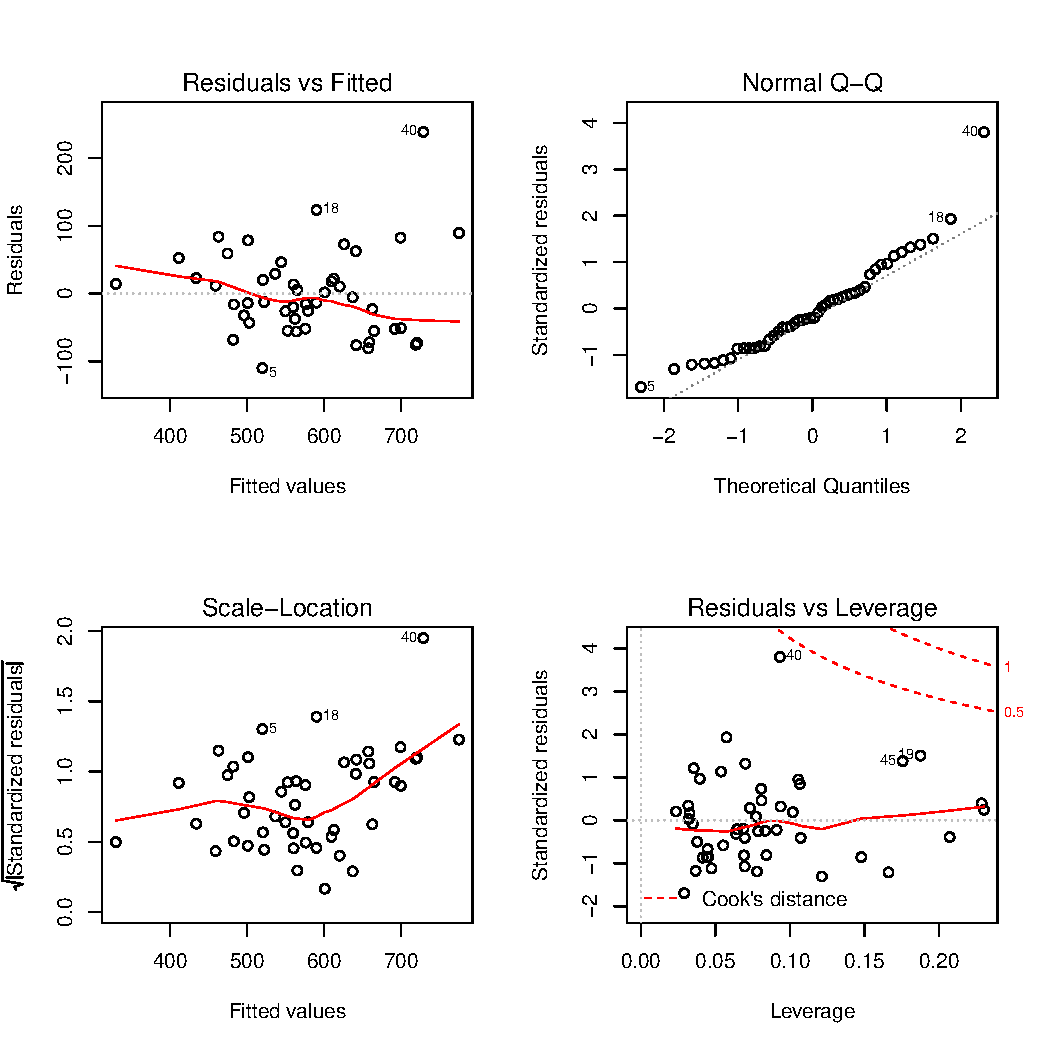
\includegraphics{Clase-6_files/figure-latex/unnamed-chunk-6-1.pdf}

\hypertarget{right}{}
\begin{itemize}
\tightlist
\item
  El grupo formado por las empresas E7 y E8, que, con inversiones
  también elevadas, si que han logrado, por el contrario, rentabilizar
  su inversión en términos de ventas.
\end{itemize}

¿Cómo se han obtenido los grupos anteriores? De una manera intuitiva
hemos visto, por ejemplo, que la empresa E1 esta a una distancia menor
de E2 que de E3 o que de cualquiera de las empresas restantes, y las
hemos puesto en un mismo grupo.

\subsection{Ejemplo}\label{ejemplo-6}

\hypertarget{left}{}
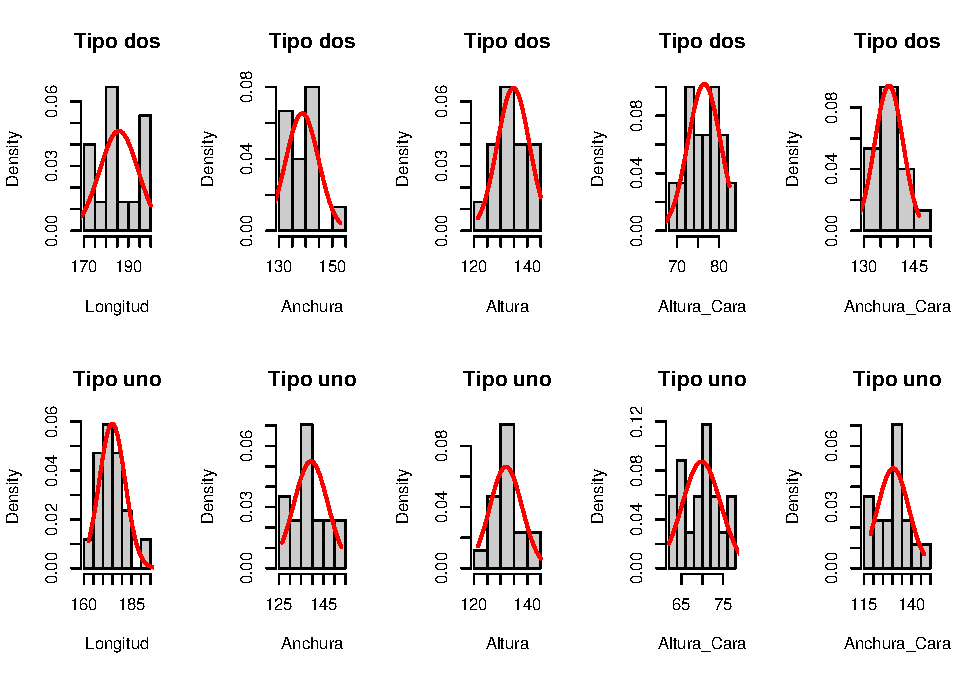
\includegraphics{Clase-6_files/figure-latex/unnamed-chunk-7-1.pdf}

\hypertarget{right}{}
De manera análoga, e igualmente intuitiva, hemos procedido con las demas
empresas, llegando a la solución de cuatro grupos expuesta. Pero ¿qué
hubiera ocurrido si en lugar de dos variables pretendiésemos llevar a
cabo agrupaciones de observaciones teniendo en cuenta 5, 10 o 50
variables?

\subsection{Ejemplo}\label{ejemplo-7}

\hypertarget{left}{}
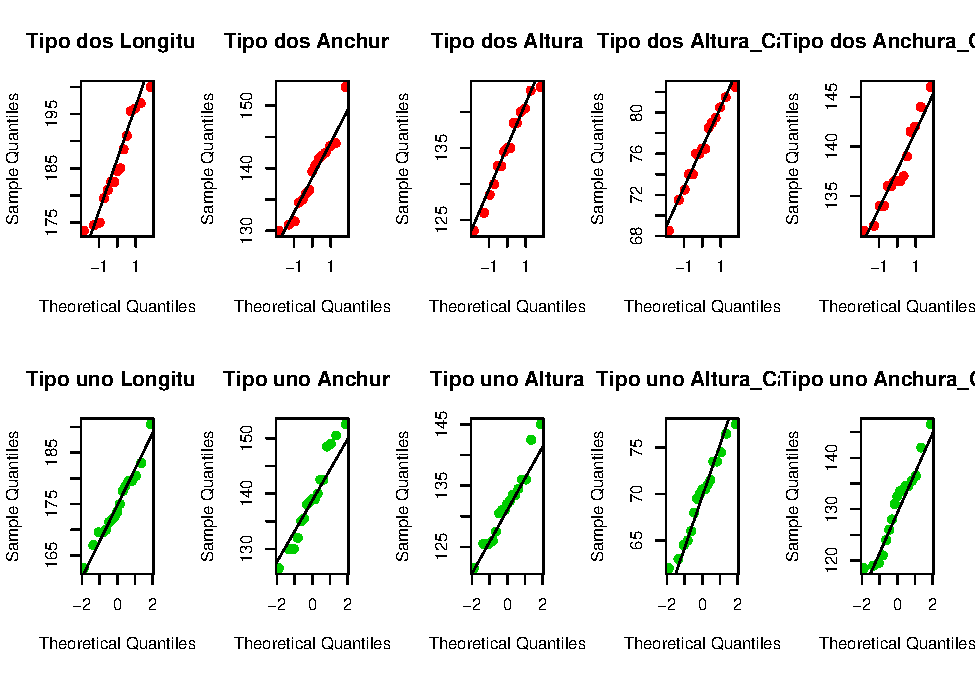
\includegraphics{Clase-6_files/figure-latex/unnamed-chunk-8-1.pdf}

\hypertarget{right}{}
La intuición debe dejar paso a la formalización. Sin embargo,
ilustraremos el proceso que sigue el análisis de conglomerados con este
ejemplo sencillo para, finalmente, aplicarlo a una situación más real en
el último epígrafe del capítulo.

Lo primero que se ha hecho de manera intuitiva es ver que E1 esta mas
cerca de E2 que de E3. Este ``más cerca'' se traduce en el análisis de
conglomerados en el cálculo de alguna medida de proximidad o similaridad
entre cada par de observaciones.

\subsection{Medidas de similaridad para variables
métricas}\label{medidas-de-similaridad-para-variables-muxe9tricas}

 En el caso en que las variables que se utilizan para caracterizar las
observaciones sean métricas, es decir, de intervalo o de razón, se puede
recurrir a cualquiera de las siguientes medidas de similaridad.
\textbf{Distancia euclídea} Si consideramos dos observaciones \(i\) y
\(j\) de las \(n\) posibles y si llamamos \(x_{ip}\) y \(x_{jp}\) al
valor que toma la variable \(x_p\), de las \(k\) existentes en dichas
observaciones, la distancia euclídea \(D_{ij}\) entre ambas se
calcularia del siguiente modo:
\[D_{ij}=\sqrt{\sum_{p=1}^{k}(x_{ip}-x_{jp})^2}\]

\subsection{Medidas de similaridad para variables
métricas}\label{medidas-de-similaridad-para-variables-muxe9tricas-1}

\hypertarget{left}{}
\begin{verbatim}
datos
\end{verbatim}

\begin{verbatim}
##    Inversion_publicitaria Ventas
## E1                     16     10
## E2                     12     14
## E3                     10     22
## E4                     12     25
## E5                     45     10
## E6                     50     15
## E7                     45     25
## E8                     50     27
\end{verbatim}

\hypertarget{right}{}
asi, por ejemplo, la distancia euclidea entre las empresas E1 y E2
tomael valor siguiente:

\[D_{12}=\sqrt{(16-12)^2+(10-14)^2}=5.66\] que es menor que la distancia
existente entre las empresas E1 y E3:

\[D_{13}=\sqrt{(16-10)^2+(10-22)^2}=13.42\]

\subsection{Ejemplo}\label{ejemplo-8}

\hypertarget{left}{}
\begin{verbatim}
# Distancia euclidiana
matriz.dis.euclid <- dist(datos[,1:2],method="euclidian",diag=TRUE)
round(matriz.dis.euclid,2)
\end{verbatim}

\begin{verbatim}
##       E1    E2    E3    E4    E5    E6    E7    E8
## E1  0.00                                          
## E2  5.66  0.00                                    
## E3 13.42  8.25  0.00                              
## E4 15.52 11.00  3.61  0.00                        
## E5 29.00 33.24 37.00 36.25  0.00                  
## E6 34.37 38.01 40.61 39.29  7.07  0.00            
## E7 32.65 34.79 35.13 33.00 15.00 11.18  0.00      
## E8 38.01 40.16 40.31 38.05 17.72 12.00  5.39  0.00
\end{verbatim}

\hypertarget{right}{}
La mayoria de algoritmos calculan las distancias entre todos los pares
de observaciones, como paso inicial del análisis de conglomerados.
Mostramos la matriz euclidiana obtenida con el R con la función
\texttt{dis()}

\subsection{Medidas de similaridad para variables
métricas}\label{medidas-de-similaridad-para-variables-muxe9tricas-2}

 \textbf{Distancia de Minkowski} Las distancia euclídea y distancia
eucídea al cuadrado son un caso particular de la distancia de Minkowski,
que viene dada porla expresión:
\[D_{ij}=[\sum_{p=1}^{k}|x_{ip}-x_{jp}|^n]^{1/n}\] Puede comprobarse que
haciendo \(n = 2\) se obtiene la expresién correspondiente a la
distancia euclídea.

\subsection{Medidas de similaridad para variables
métricas}\label{medidas-de-similaridad-para-variables-muxe9tricas-3}

 \textbf{Distancia city block o ``Manhattan''} Si en la expresion de la
distancia de Minkowski tomaramos \(n = 1\), obtendríamos la denominada
distancia city block, la cuál viene dada por:
\[D_{ij}=\sum_{p=1}^{k}|x_{ip}-x_{jp}|\]

\subsection{Estandarización de los
datos}\label{estandarizaciuxf3n-de-los-datos}

 Si se analizan con detenimiento las medidas de distancia presentadas,
se puede comprobar que todas ellas estén basadas en la sustracción, para
cada par de observaciones, de los valores de las variables utilizadas en
su caracterización. Por ello, se puede esperar que las medidas de
disimilaridad sean muy sensibles a las unidades en que estén medidas
dichas variables. Si pretendemos agrupar empresas en función de dos
variables, como el tamaño de su activos medido en pesetas y el número de
trabajadores, la primera variable contribuirá mucho mas a establecer los
grupos que la segunda. Y esto no se debe a que conceptualmente una sea
mucho mas importante que la otra, sino a que, con esas unidades, su
valor absoluto será siempre muy superior.

\subsection{Estandarización de los
datos}\label{estandarizaciuxf3n-de-los-datos-1}

\hypertarget{left}{}
\begin{verbatim}
nombre.empresa2<-c("E1","E2","E3","E4","E5","E6","E7","E8")
activos<-c(10.0e9,10.5e9,10.0e9,10.5e9,20.0e9,20.5e9,20.0e9,20.5e9)
trabajadores<-c(100,90,200,190,200,190,100,90)
Datos_EST<-data.frame(nombre.empresa2,activos,trabajadores)
Datos_EST
\end{verbatim}

\begin{verbatim}
##   nombre.empresa2  activos trabajadores
## 1              E1 1.00e+10          100
## 2              E2 1.05e+10           90
## 3              E3 1.00e+10          200
## 4              E4 1.05e+10          190
## 5              E5 2.00e+10          200
## 6              E6 2.05e+10          190
## 7              E7 2.00e+10          100
## 8              E8 2.05e+10           90
\end{verbatim}

\hypertarget{right}{}
Los datos presentados recogen el tamaño de los activos y el número de
trabajadores de ocho empresas hipotéticas. Si efectuamos un análisis de
conglomerados con las unidades originales, la matriz de distancias
mostrará que los dos grupos obtenidos responden exclusivamente a la
variable ``activos de la empresa'', puesto que sitúa en un mismo grupo a
aquellas con cifras que rondan los 10000 millones de pesetas (E1, E2, E3
y E4) y en otro grupo a las que tienen activos en torno a los 20000
millones (E5, E6, E7 y E8).

\subsection{Estandarización de los
datos}\label{estandarizaciuxf3n-de-los-datos-2}

\hypertarget{left}{}
\begin{verbatim}
matriz.dis.euclid2<-dist(Datos_SEST[,c("activos","trabajadores")],method="euclidean",diag=TRUE)
matriz.dis.euclid2
\end{verbatim}

\begin{verbatim}
##          1        2        3        4        5        6        7        8
## 1 0.00e+00                                                               
## 2 5.00e+08 0.00e+00                                                      
## 3 1.00e+02 5.00e+08 0.00e+00                                             
## 4 5.00e+08 1.00e+02 5.00e+08 0.00e+00                                    
## 5 1.00e+10 9.50e+09 1.00e+10 9.50e+09 0.00e+00                           
## 6 1.05e+10 1.00e+10 1.05e+10 1.00e+10 5.00e+08 0.00e+00                  
## 7 1.00e+10 9.50e+09 1.00e+10 9.50e+09 1.00e+02 5.00e+08 0.00e+00         
## 8 1.05e+10 1.00e+10 1.05e+10 1.00e+10 5.00e+08 1.00e+02 5.00e+08 0.00e+00
\end{verbatim}

\hypertarget{right}{}
Es decir, la influencia del número de trabajadores en la obtención de
estos conglomerados es practicamente nula. Para evitar esta influencia
no deseable de una variable debida exclusivamente a la unidad en que
viene medida es necesario corregir el efecto de los datos recurriendo a
un proceso de estandarización.

\subsection{Estandarización de los
datos}\label{estandarizaciuxf3n-de-los-datos-3}

 \textbf{Puntuaciones Z} Los datos son estandarizados, restando al valor
de cada observación de una variable determinada,la media de esa variable
para el conjunto de las observaciones y dividiendo el resultado por su
desviación típica. De esta forma la variable estandarizada tiene media
0, y desviación típica, 1. \textbf{Rango 1} El valor de una variable
dada en cada observación es dividido por el rango de esa variable para
el conjunto de observaciones. De esta forma el rango de variación de la
variable así estandarizada queda reducido a un intervalo de valor 1.

\subsection{Estandarización de los
datos}\label{estandarizaciuxf3n-de-los-datos-4}

\textbf{Rango 0 a 1} El valor de una variable determinada para cada
observación es estandarizada sustrayéndole el valor mínimo que toma esa
variable en el conjunto de las observaciones y a continuación dividiendo
por el rango. De esta forma el valor mínimo de las variables sera 0, y
el máximo, 1.

\subsection{Estandarización de los
datos}\label{estandarizaciuxf3n-de-los-datos-5}

\hypertarget{left}{}
\begin{verbatim}
Datos_EST<-scale(Datos_SEST[,c("activos","trabajadores")])
matriz.dis.euclid.norm<-dist(Datos_EST[,c("activos","trabajadores")],method="euclidean",diag=TRUE)
round(matriz.dis.euclid.norm,2)
\end{verbatim}

\begin{verbatim}
##      1    2    3    4    5    6    7    8
## 1 0.00                                   
## 2 0.21 0.00                              
## 3 1.86 2.05 0.00                         
## 4 1.68 1.86 0.21 0.00                    
## 5 2.64 2.71 1.87 1.78 0.00               
## 6 2.58 2.64 1.97 1.87 0.21 0.00          
## 7 1.87 1.78 2.64 2.44 1.86 1.68 0.00     
## 8 1.97 1.87 2.84 2.64 2.05 1.86 0.21 0.00
\end{verbatim}

\hypertarget{right}{}
Veamos si estandarizando los datos del ejemplo mediante el procedimiento
de las puntuaciones Z, se logra corregir la influencia desproporcionada
de la variable activos de la empresa en la formación de los grupos.
Usaremos para ello la función \texttt{scale\{base\}}.

\subsection{Estandarización de los
datos}\label{estandarizaciuxf3n-de-los-datos-6}

\hypertarget{left}{}
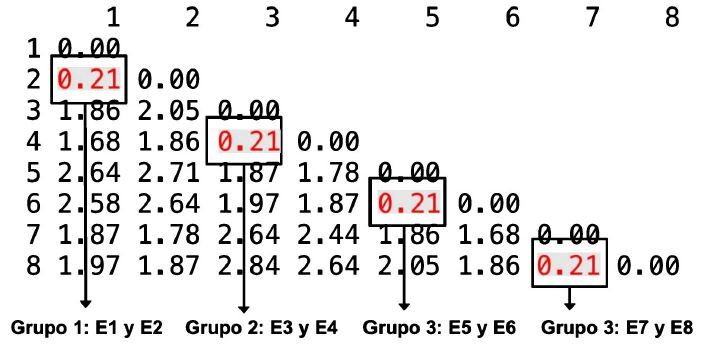
\includegraphics[width=1\linewidth]{images/dist_est}

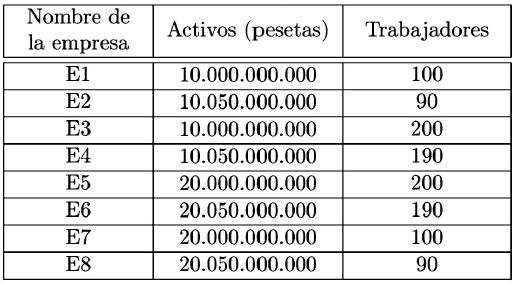
\includegraphics[width=1\linewidth]{images/empresa}

\hypertarget{right}{}
Ahora aparecen cuatro grupos formados por dos empresas que se parecen
mucho entre sí. Asi, el formado por E1 y E2 tienen activos en torno a
los 10.000 millones, pero los separa del grupo formado por E3 y E4 el
hecho de que estas últimas empresas les doblan en términos de número de
trabajadores. Se observa como, estandarizando los datos, se elimina el
efecto de las unidades de medida y las dos variables que caracterizan
las observaciones tienen el mismo peso a la hora de formar los grupos.

\subsection{Formación de los grupos}\label{formaciuxf3n-de-los-grupos}

 Los algoritmos de agrupación existentes responden a dos grandes
enfoques: \textbf{Métodos jerárquicos:} Existen dos enfoques *
\emph{Métodos jerárquicos aglomerativos}: inicialmente cada individuo es
un grupo en sí mismo. Sucesivamente se van formando grupos de mayor
tamaño fusionando grupos cercanos entre sí. Finalmente, todos los
individuos confluyen en un solo grupo.

\begin{itemize}
\tightlist
\item
  \emph{Métodos jerarquicos desagregativos}: inicialmente, todos los
  individuos forman un único grupo y se van sucesivamente desgajando de
  él, formando dos grupos, tres grupos y asi hasta que al final del
  proceso cada caso forma un único grupo.
\end{itemize}

La mayoría de paquetes estadísticos usan el primer enfoque.

\subsection{Principales algoritmos de agrupamiento
jerárquico}\label{principales-algoritmos-de-agrupamiento-jeruxe1rquico}

 \textbf{Método del centroide}

\begin{itemize}
\tightlist
\item
  Está implementado en la función de \texttt{R},
  \texttt{hclust\{stats\}}.
\item
  En primer lugar, se calcula la matriz de distancias, en este caso
  euclidea al cuadrado, entre las ocho empresas usando el siguiente
  código de R. 
\end{itemize}

\begin{verbatim}
library(stats)
#calculo de la distancia euclídea
matriz.dis.euclid<-dist(datos[,c("Inversion_publicitaria","Ventas")],method="euclidean",diag=TRUE)

#calculo de la distancia euclidea al cuadrado
matriz.dis.euclid2<-(matriz.dis.euclid)^2
matriz.dis.euclid2
\end{verbatim}

\subsection{Método del centroide}\label{muxe9todo-del-centroide}

\hypertarget{left}{}
\begin{verbatim}
##      E1   E2   E3   E4   E5   E6   E7   E8
## E1    0                                   
## E2   32    0                              
## E3  180   68    0                         
## E4  241  121   13    0                    
## E5  841 1105 1369 1314    0               
## E6 1181 1445 1649 1544   50    0          
## E7 1066 1210 1234 1089  225  125    0     
## E8 1445 1613 1625 1448  314  144   29    0
\end{verbatim}

\hypertarget{right}{}
\begin{itemize}
\tightlist
\item
  Se puede apreciar la matriz de distancias euclídeas al cuadrado.
\item
  En esta matriz se puede apreciar que las empresas más cercanas son E3
  y E4.
\end{itemize}

\subsection{Método del centroide}\label{muxe9todo-del-centroide-1}

\hypertarget{left}{}
\begin{verbatim}
#efectuamos el cluster con método centroide
hclust.centroide<-hclust(matriz.dis.euclid2,method="centroid")

#Saca el historial de aglomeración del objeto hclust.centroide
data.frame(hclust.centroide[2:1])
\end{verbatim}

\begin{verbatim}
##    height merge.1 merge.2
## 1   13.00      -3      -4
## 2   29.00      -7      -8
## 3   32.00      -1      -2
## 4   50.00      -5      -6
## 5  141.25       1       3
## 6  182.25       2       4
## 7 1227.25       5       6
\end{verbatim}

\hypertarget{right}{}
\begin{itemize}
\tightlist
\item
  Pues bien, el método del centroide comienza uniendo aquellas dos
  observaciones que estén més cercanas, en este caso las empresas E3 y
  E4 (la distancia es 13).
\item
  A continuación el grupo formado es sustituido por una observación que
  lo representa y en la que las variables toman los valores medios de
  todas las observaciones que constituyen el grupo representado
  (centroide).
\item
  En nuestro ejemplo, las empresas E3 y E4 son sustituidas por una
  empresa promedio, que
\end{itemize}

\subsection{Método del centroide}\label{muxe9todo-del-centroide-2}

\hypertarget{left}{}
\begin{verbatim}
datos
\end{verbatim}

\begin{verbatim}
##    Inversion_publicitaria Ventas
## E1                     16     10
## E2                     12     14
## E3                     10     22
## E4                     12     25
## E5                     45     10
## E6                     50     15
## E7                     45     25
## E8                     50     27
\end{verbatim}

\hypertarget{right}{}
En nuestro ejemplo, las empresas E3 y E4 son sustituidas por una empresa
promedio, que llamaremos E3-4, para la que el gasto en publicidad y las
ventas toman los siguientes valores:
\[Publicidad-E3-4=\frac{10+12}{2}=11\]
\[Ventas-E3-4=\frac{22+25}{2}=23.5\] En ese momento se recalcula la
matriz de distancias, solo que, en lugar de estar presentes las empresas
E3 y E4, esta su centroide E3-4.

\subsection{Método del centroide}\label{muxe9todo-del-centroide-3}

\hypertarget{left}{}
\begin{verbatim}
#efectuamos el cluster con método centroide
hclust.centroide<-hclust(matriz.dis.euclid2,method="centroid")

#Saca el historial de aglomeración del objeto hclust.centroide
data.frame(hclust.centroide[2:1])
\end{verbatim}

\begin{verbatim}
##    height merge.1 merge.2
## 1   13.00      -3      -4
## 2   29.00      -7      -8
## 3   32.00      -1      -2
## 4   50.00      -5      -6
## 5  141.25       1       3
## 6  182.25       2       4
## 7 1227.25       5       6
\end{verbatim}

\hypertarget{right}{}
\begin{itemize}
\tightlist
\item
  \texttt{hclust} muestra esas distancias sucesivas en lo que
  denominamos el historial de conglomeración.
\item
  En el paso 5 se fusionan las empresas que lo hicieron en el paso 1
  (E3-4) con las quelo hicieron en el paso 3 (E1-2).
\item
  El proceso termina cuando todas las empresas estan en un solo grupo.
\end{itemize}

\subsection{Método del centroide}\label{muxe9todo-del-centroide-4}

\hypertarget{left}{}
\begin{verbatim}
#dendograma centroide
plot.hclust<-plot(hclust.centroide)
rect.hclust(hclust.centroide, k = 2, border = "red")
\end{verbatim}

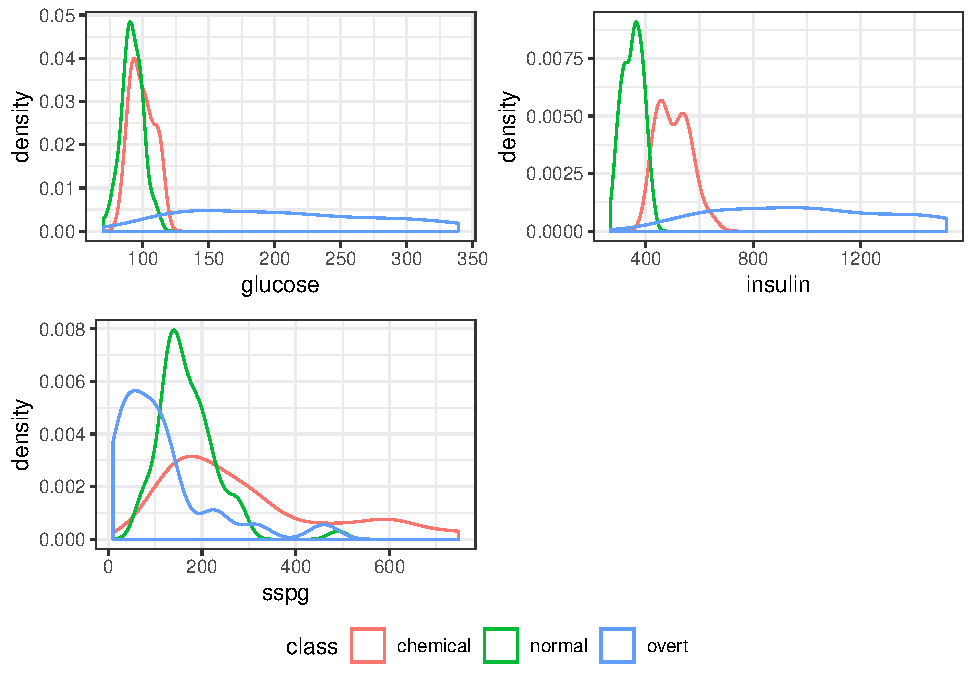
\includegraphics{Clase-6_files/figure-latex/unnamed-chunk-20-1.pdf}

\hypertarget{right}{}
\begin{itemize}
\tightlist
\item
  El historial de conglomeración tiene una traducción gráfica que es de
  gran utilidad para determinar el número razonable de grupos que debe
  retenerse.
\item
  A este gráfico se le denomina \emph{dendograma}.
\item
  Obsérvese como los grupos que se formaron en la etapa 5 (empresas 3,
  4, 1 y 2) y los que se formaronenla 6 (7, 8, 5 y 6) estan a tal
  distancia que no es razonable fusionarlos. Esos dos grupos son los que
  el analista deberia retener.
\end{itemize}


\end{document}
